
%\section{Question 1}
\textbf{Simulate the saturation behaviour of a dynamo from helically forced turbulence with forcing wave-number $k_f = 3$ in units of the box wave-number $k_1 = 1$.}

During  this question I will use the example configuration \texttt{samples/helical-MHDturb}, changing different parameters though the questions.

\subsection{Critical value for the magnetic diffusivity.}

Calculation of the critical value for the magnetic diffusivity implies running the code for different values of the magnetic diffusivity and checking up at which value the field starts growing.

Since the proposed value for $\eta$ ($\eta = 2e-3$) corresponds to a growing field, I have tried several values bigger than the one proposed.

In figure \ref{fig:brmst} the growth of the rms magnetic field versus time can be analyzed for different magnetic diffusivity values.

\begin{figure}[h]
\centering
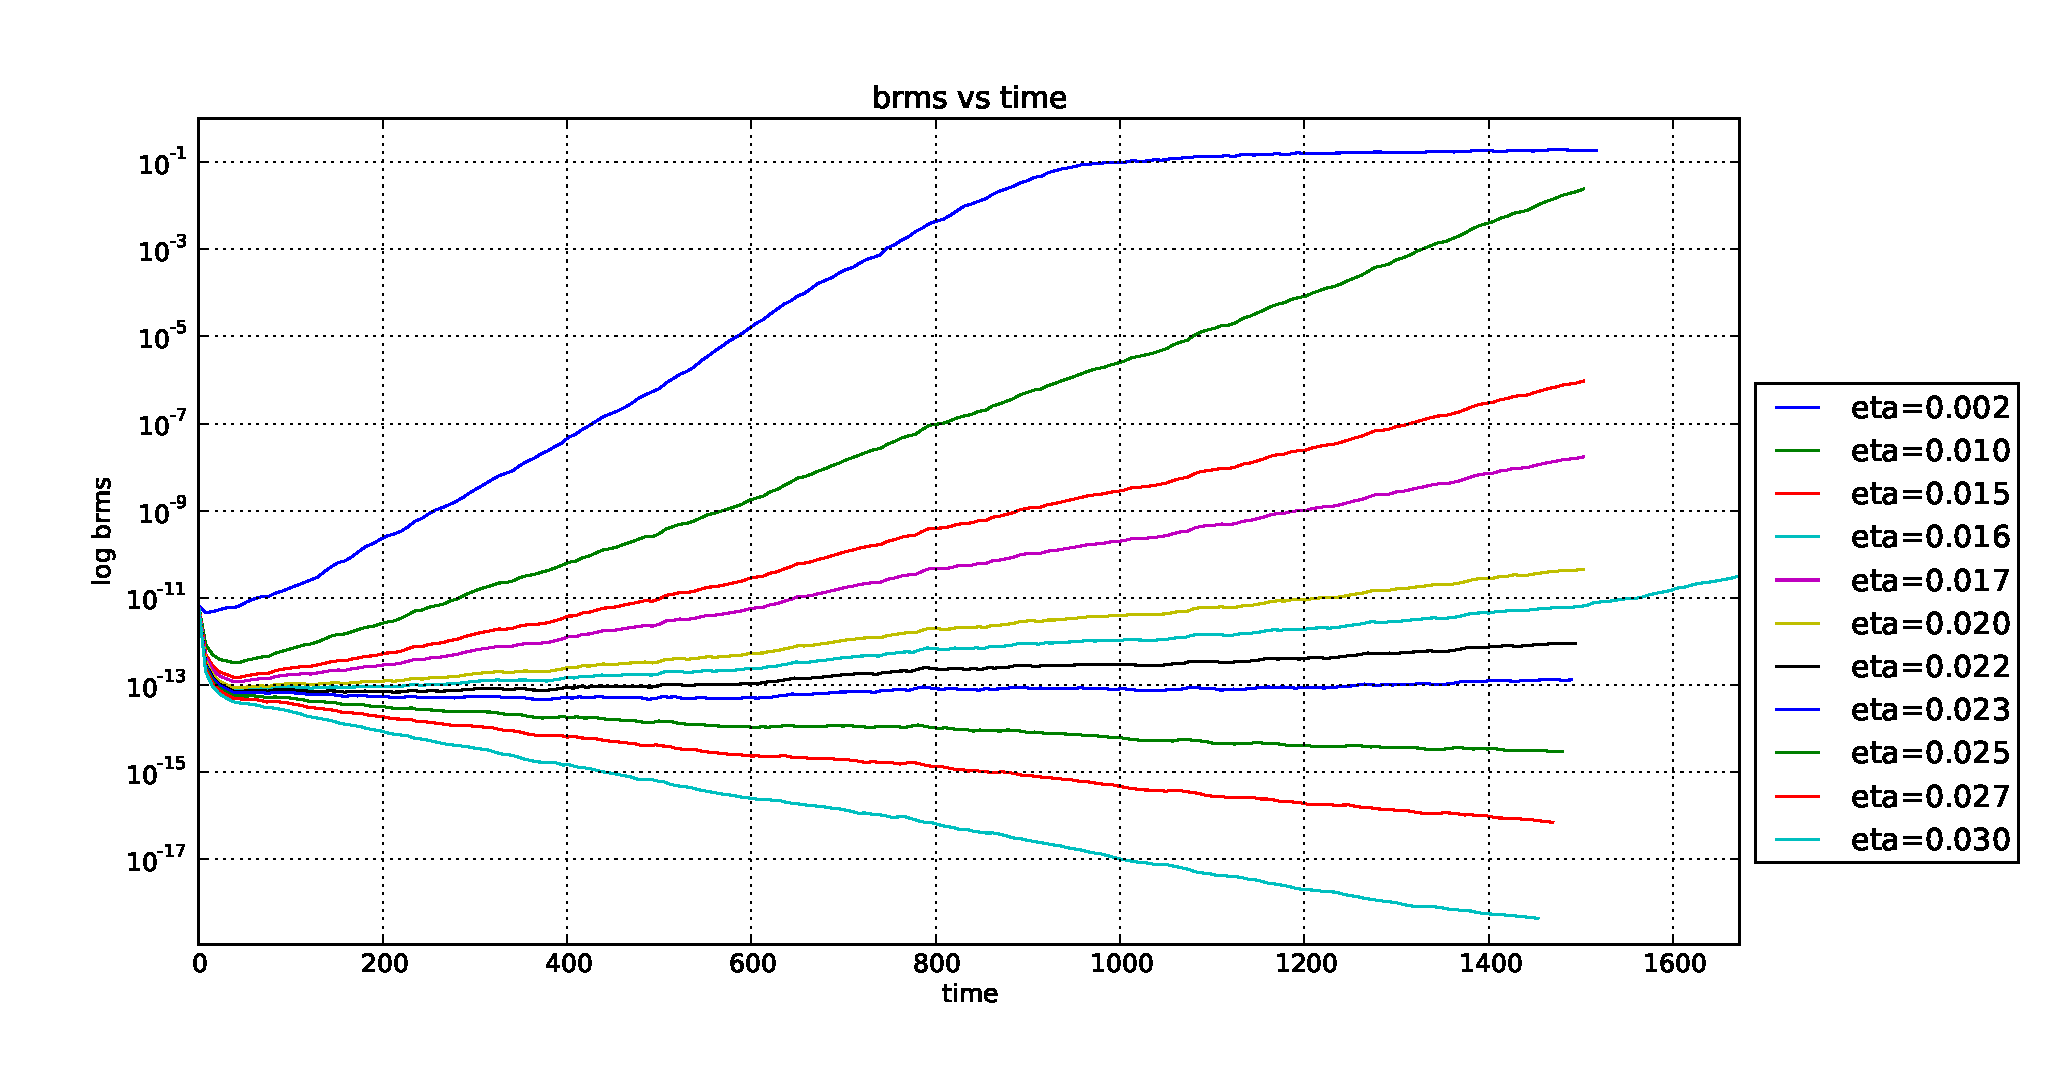
\includegraphics[width=0.8\textwidth]{brms_vs_time.eps}
\caption{log(brms) vs time for different values of  magnetic diffusivity.}
\label{fig:brmst}
 \end{figure}


I tried to find out the critical value for the magnetic diffusivity computing the first derivative of these  curves, restricted to the linear range $100 < t < 900$, and calculating the mean of each derivative. Both quantities are represented in figure \ref{fig:crit_eta}.
\begin{figure}[h]
\centering
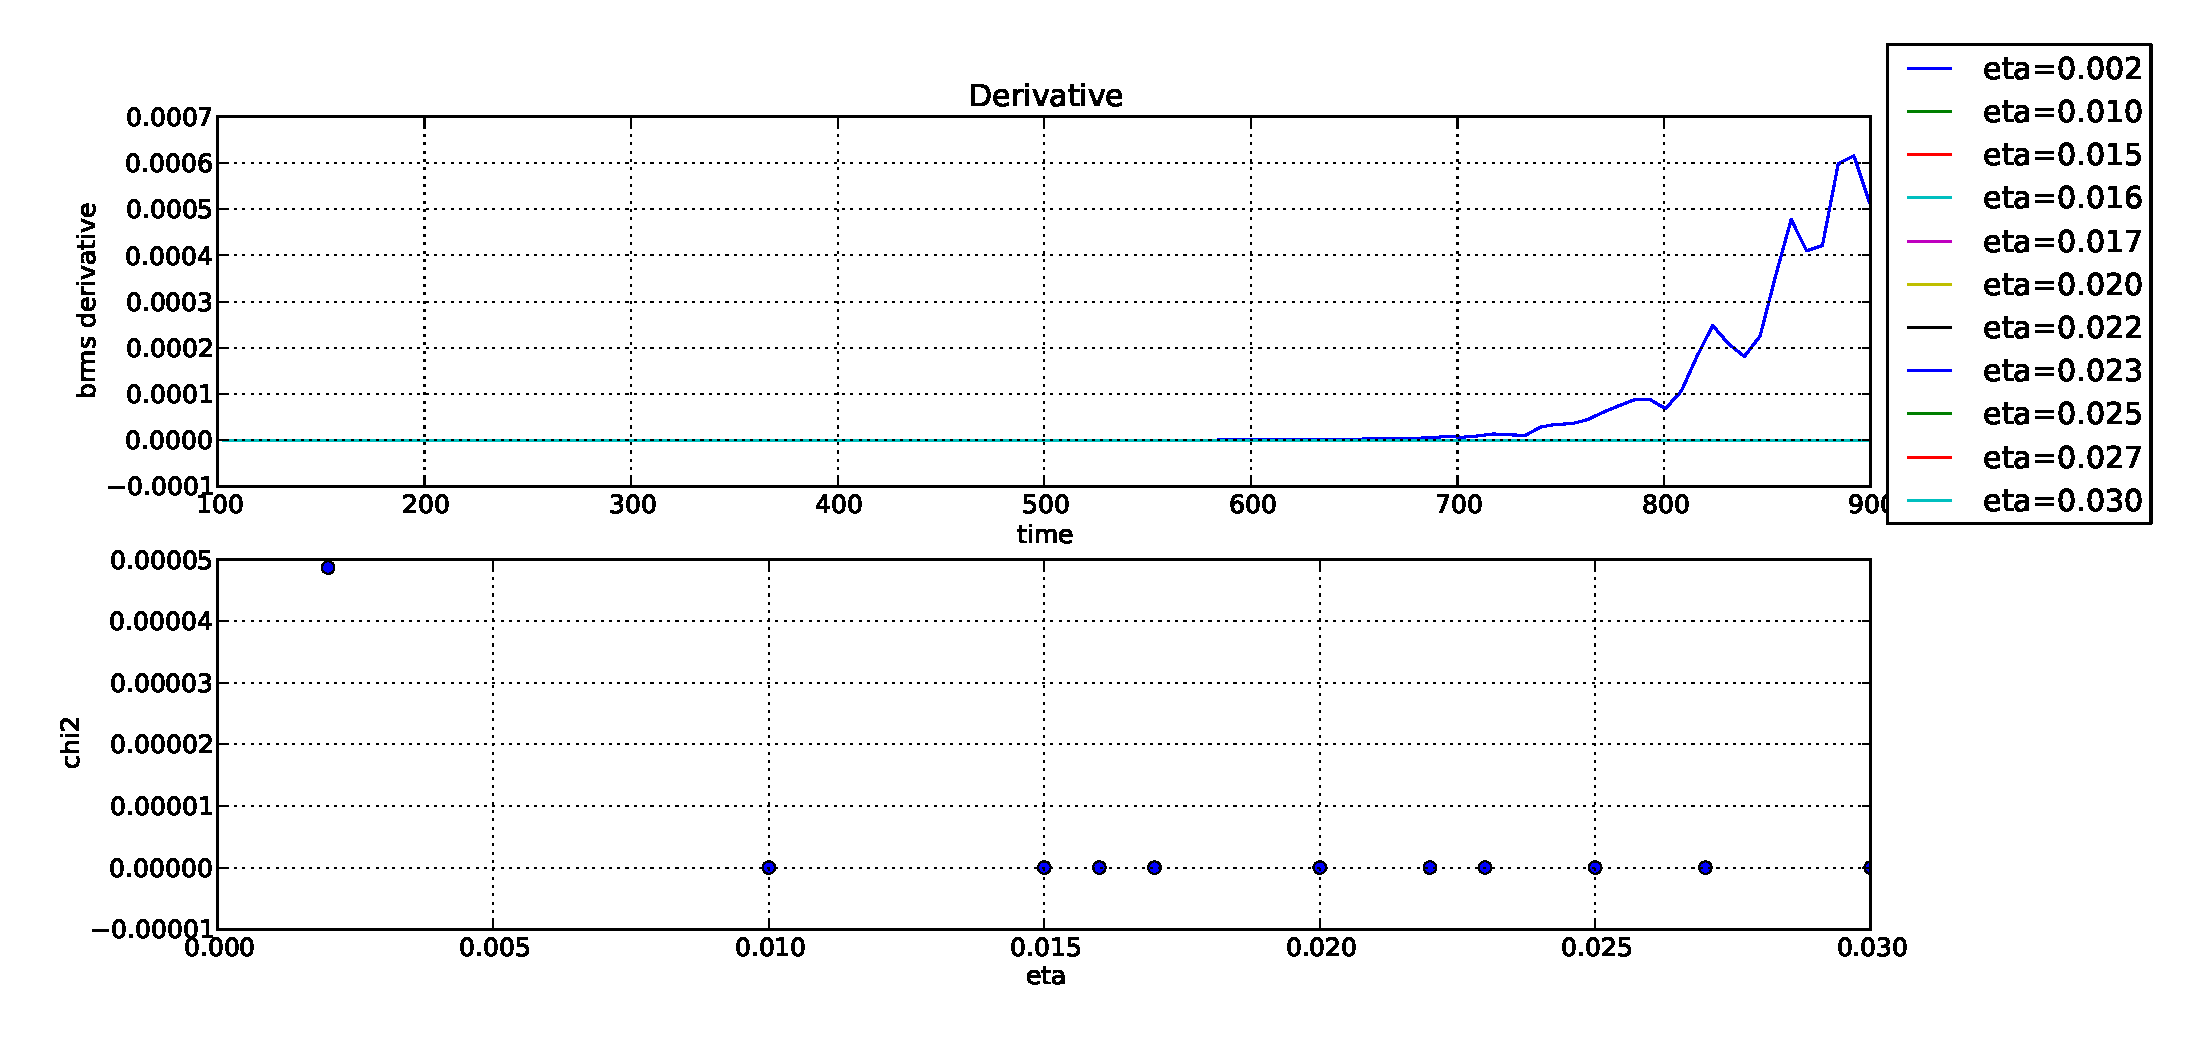
\includegraphics[width=0.8\textwidth]{critical_eta.eps}
\caption{brms derivative vs time and derivative mean for different values of the magnetic diffusivity.}
\label{fig:crit_eta}
 \end{figure}

The mean derivative of the field decreases very quickly to small values:
\begin{center}
\begin{tabular}{ll}
$\eta$ & mean(derivative)\\\hline
2e-3 & 4.87e-05\\
10e-3 & 6.89e-10\\
15e-3 & 1.48e-12\\
16e-3 & 1.04e-15\\
17e-3 & 1.33e-13\\
20e-3 & 3.63e-15\\
22e-3 & 2.63e-16\\
23e-3 & 2.52e-17\\
25e-3 & -5.09e-17\\
27e-3 & -4.54e-17\\
30e-3 & -3.07e-17\\
\end{tabular}
\end{center}

Using these results, I set the critical value for the magnetic diffusivity in $\eta = 22e-3$.

\subsection{Magnetic Reynolds number}
The magnetic Reynolds number is defined as:
\begin{equation}
 Re_M = \frac{u_{rms}}{\eta \kappa_f}
\end{equation}
In this problem I have fixed $\kappa_f = 3$, I found the critical value for the magnetic diffusivity  $\eta = 22e-3$ and the mean value for $u_{rms}$ is $\bar{u_{rms}} = 0.14$, so the corresponding magnetic Reynolds number is $Re_M = 2.15$.

The magnetic Reynolds number is the ratio between convection and diffusion. When $Re_M \gg 1$, convection dominates, whereas for $Re_M \approx 1$, or less, diffusion becomes important. So, in this exercise, diffusion is about to become important.

In fact, the next table shows that $Re_M$ decreases as $\eta$ increases:
\begin{center}
\begin{tabular}{ll}
$\eta$ & $Re_M$\\\hline
2e-3 & 22.39\\
10e-3 & 4.73\\
15e-3 & 3.16\\
16e-3 & 2.97\\
17e-3 & 2.78\\
20e-3 & 2.37\\
22e-3 & 2.15\\
23e-3 & 2.06\\
25e-3 & 1.89\\
27e-3 & 1.75\\
30e-3 & 1.58\\
\end{tabular}
\end{center}

\subsection{Growth rate of the magnetic field}

In order to determine the growth rate of the magnetic field for a value of the magnetic diffusivity, I plotted the logarithm of $brms$ versus time and I did a fit on the sloped part of the curves, as shown in the figures \ref{fig:growth2} and \ref{fig:growth10}.

\begin{figure}[h]
\begin{minipage}[t]{.45\textwidth}
\centering
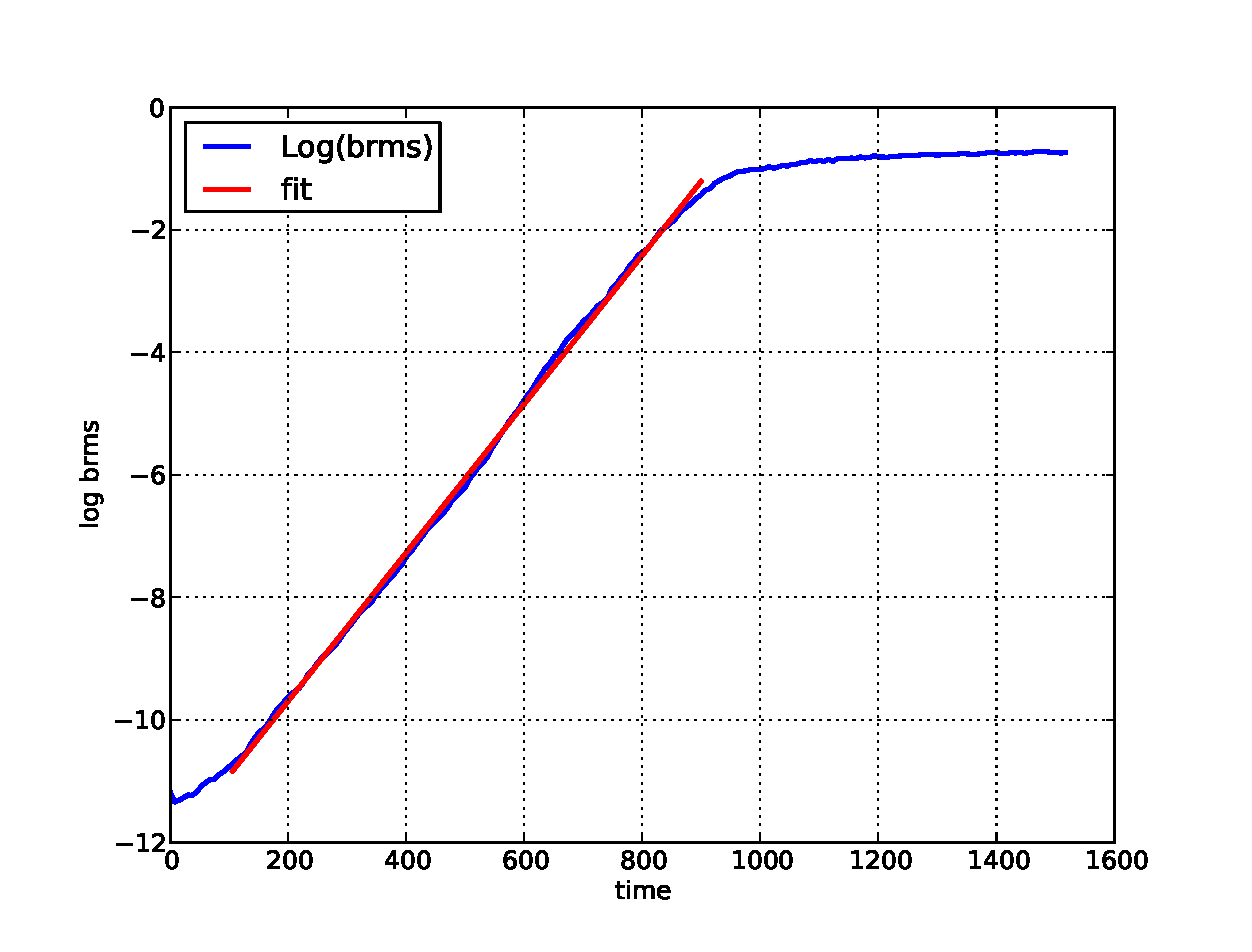
\includegraphics[width=\textwidth]{growth2e-3.eps}
\caption{Growth rate of the magnetic field for a value of the magnetic diffusivity  $\eta = 2e-3$.}
\label{fig:growth2}
\end{minipage}
\hspace{0.5cm}
\begin{minipage}[t]{.45\textwidth}
\centering
 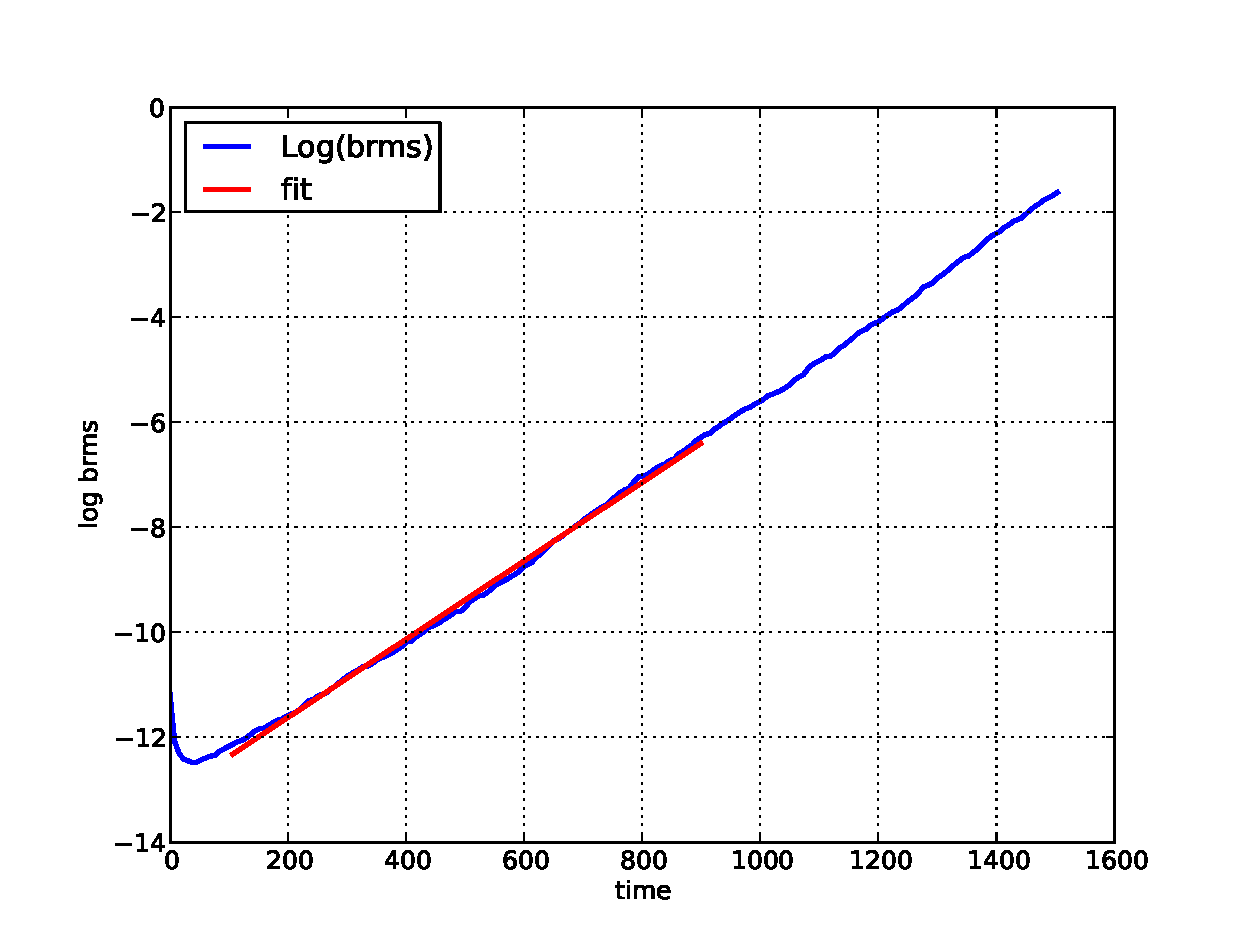
\includegraphics[width=\textwidth]{growth10e-3.eps}
\caption{Growth rate of the magnetic field for a value of the magnetic diffusivity  $\eta = 10e-3$.}
\label{fig:growth10}
\end{minipage}
 \end{figure}
%y=ax+b
The parameter $a$ in a linear regression fit ($y=ax+b$) is a measure of the growth rate of the magnetic field. The growth depends on the value of the magnetic diffusivity, and it decreases as the magnetic diffusivity increases.
\begin{center}
\begin{tabular}{lll}
$\eta$ & a & b\\\hline
2e-3 & 0.0121 & -12.12\\
10e-3 & 0.0075 & -13.11
\end{tabular}
\end{center}

\subsection{Structure of the magnetic field.}

Figure \ref{fig:averages} shows the evolution of three different magnetic field averages: the xy average bmz, the yz average bmx and the zx average bmy. 
From the figure one can see that the $zx$ average dominates in the end.
\begin{figure}[h]
\centering
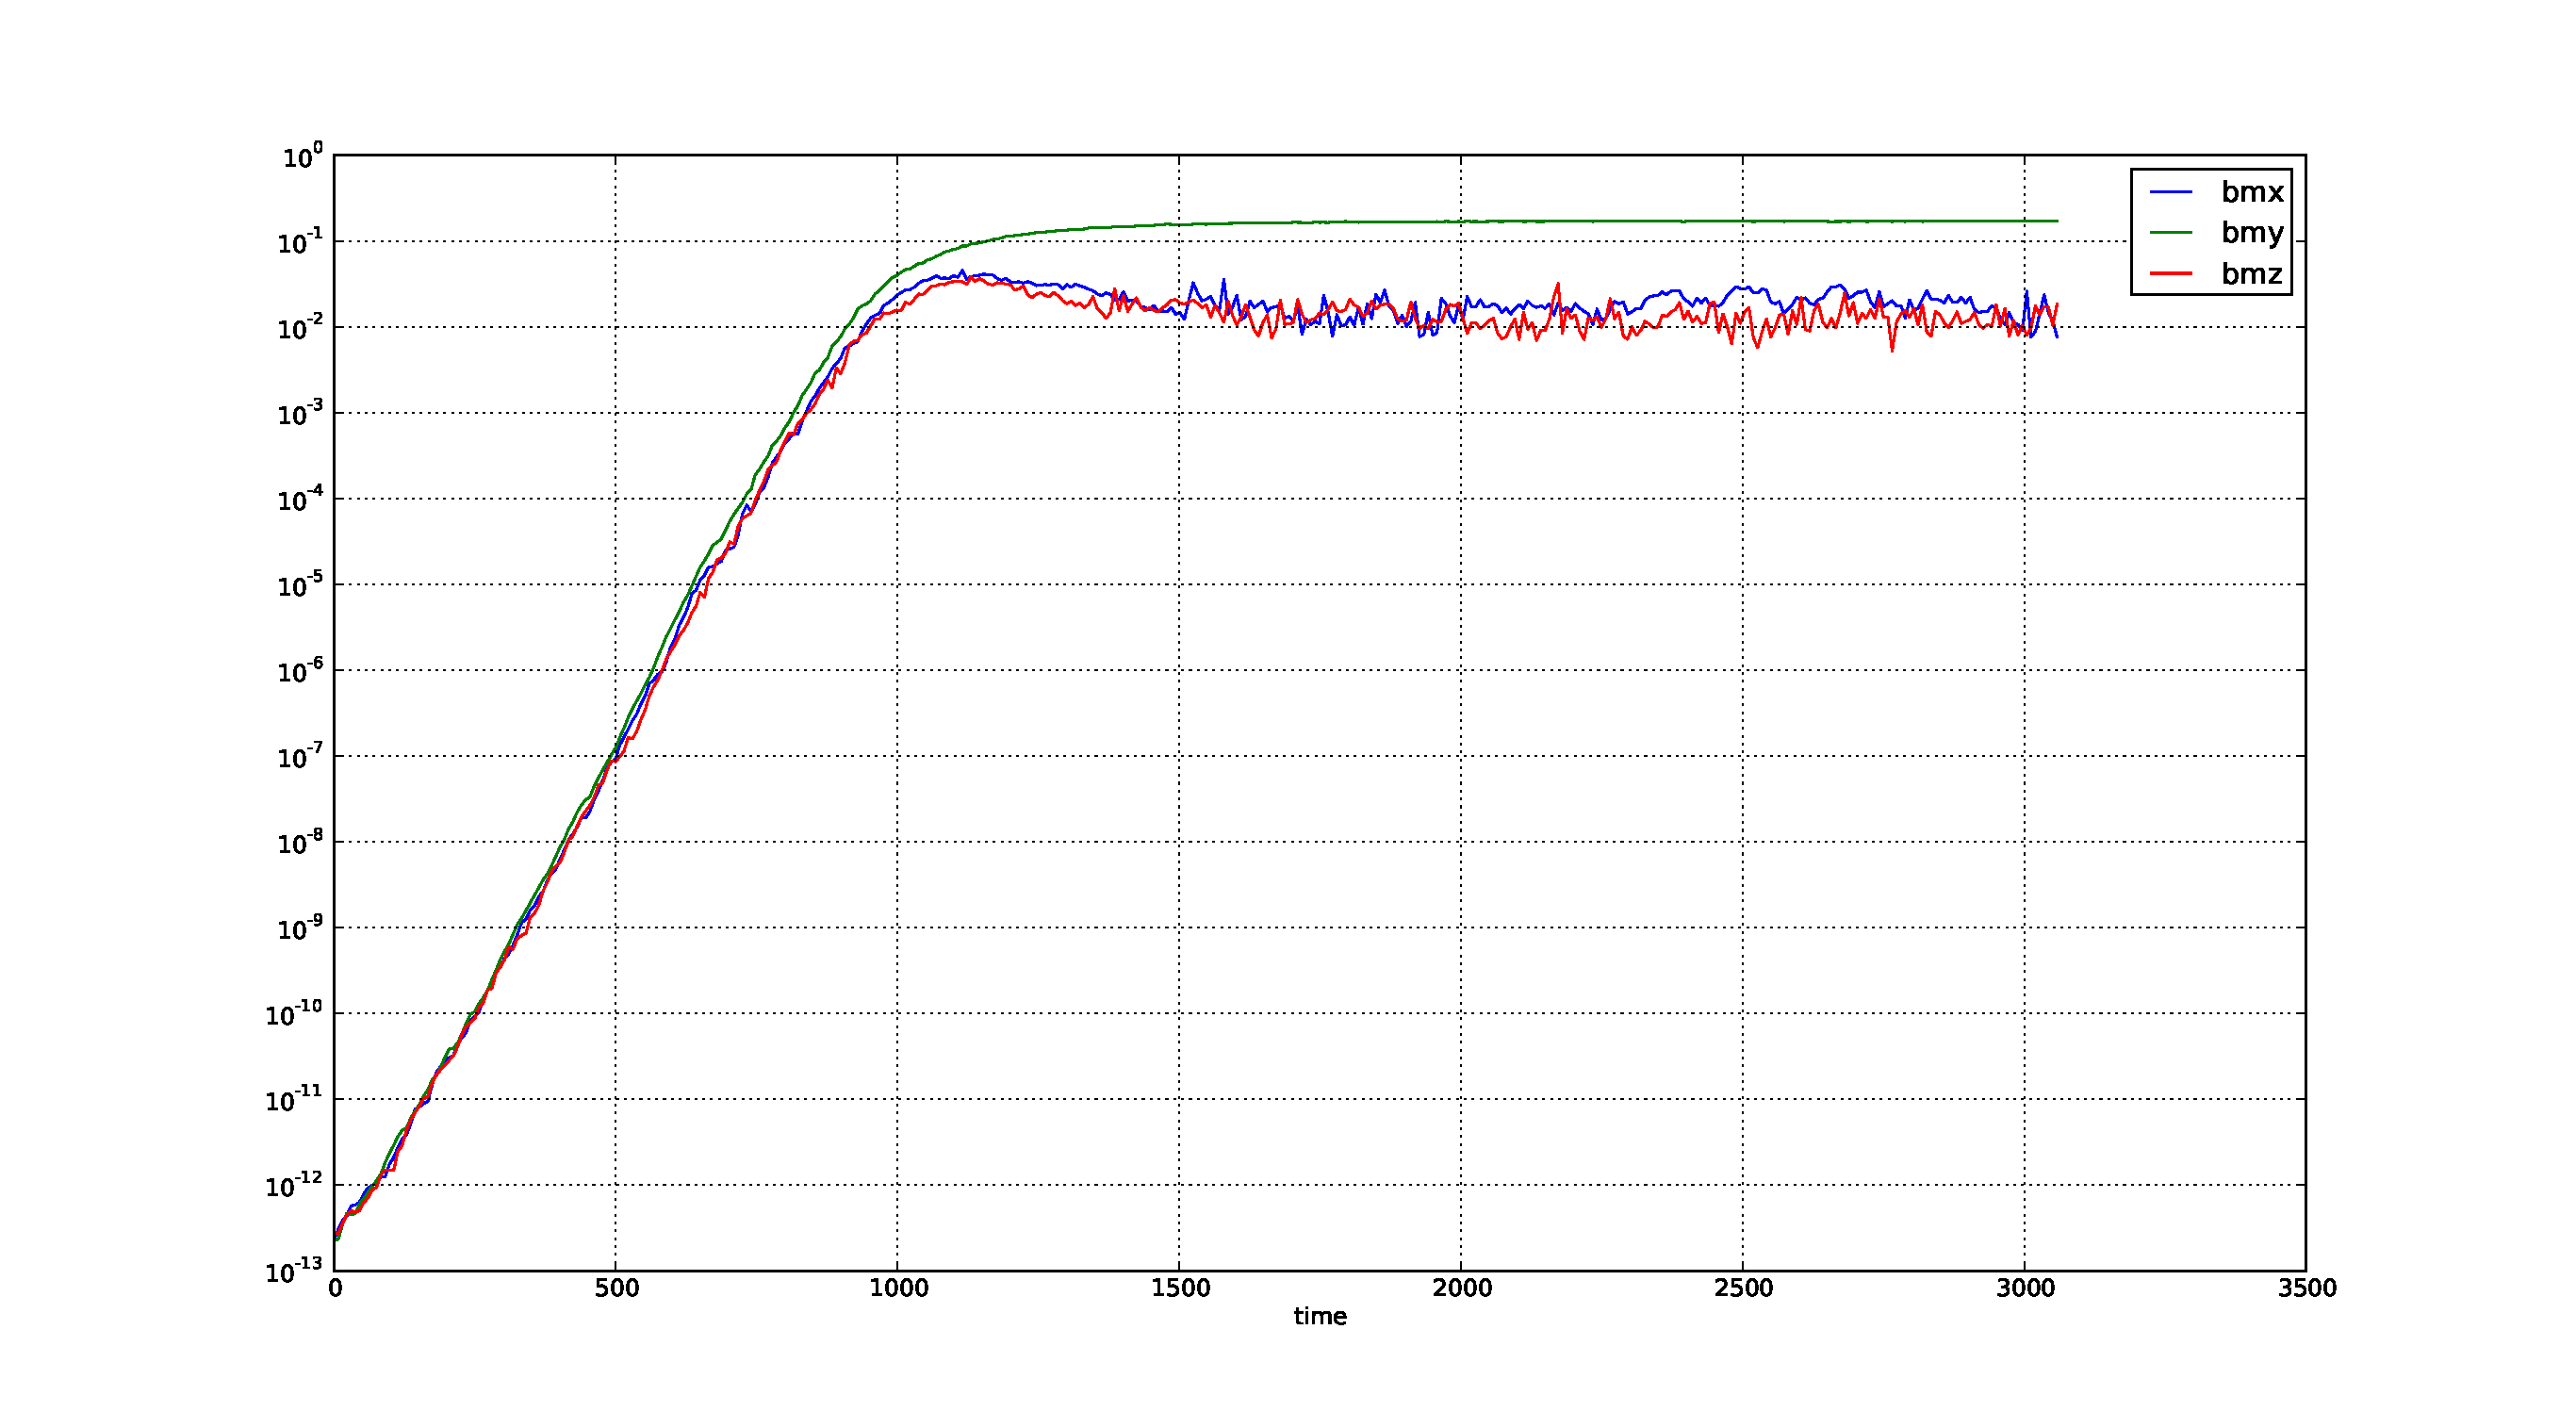
\includegraphics[width=0.8\textwidth]{campos3.eps}
\caption{Averages of three different magnetic fields.}
\label{fig:averages}
 \end{figure}

\subsection{Fitting $B_{zx}$}
Fitting the strongest of the three field averages $<\bar{B^2}>$ to the expression:
\begin{equation}
 F(t;B_0,t_s)=B_0^2[1-\exp^{-2\eta\kappa_1^2(t-t_s)}]
\label{eq:fitB}
\end{equation}
The strongest of the three field averages is the zx average represented in the figure \ref{fig:bmy_fit} with different values of the expression \ref{eq:fitB}.
\begin{figure}[h]
\centering
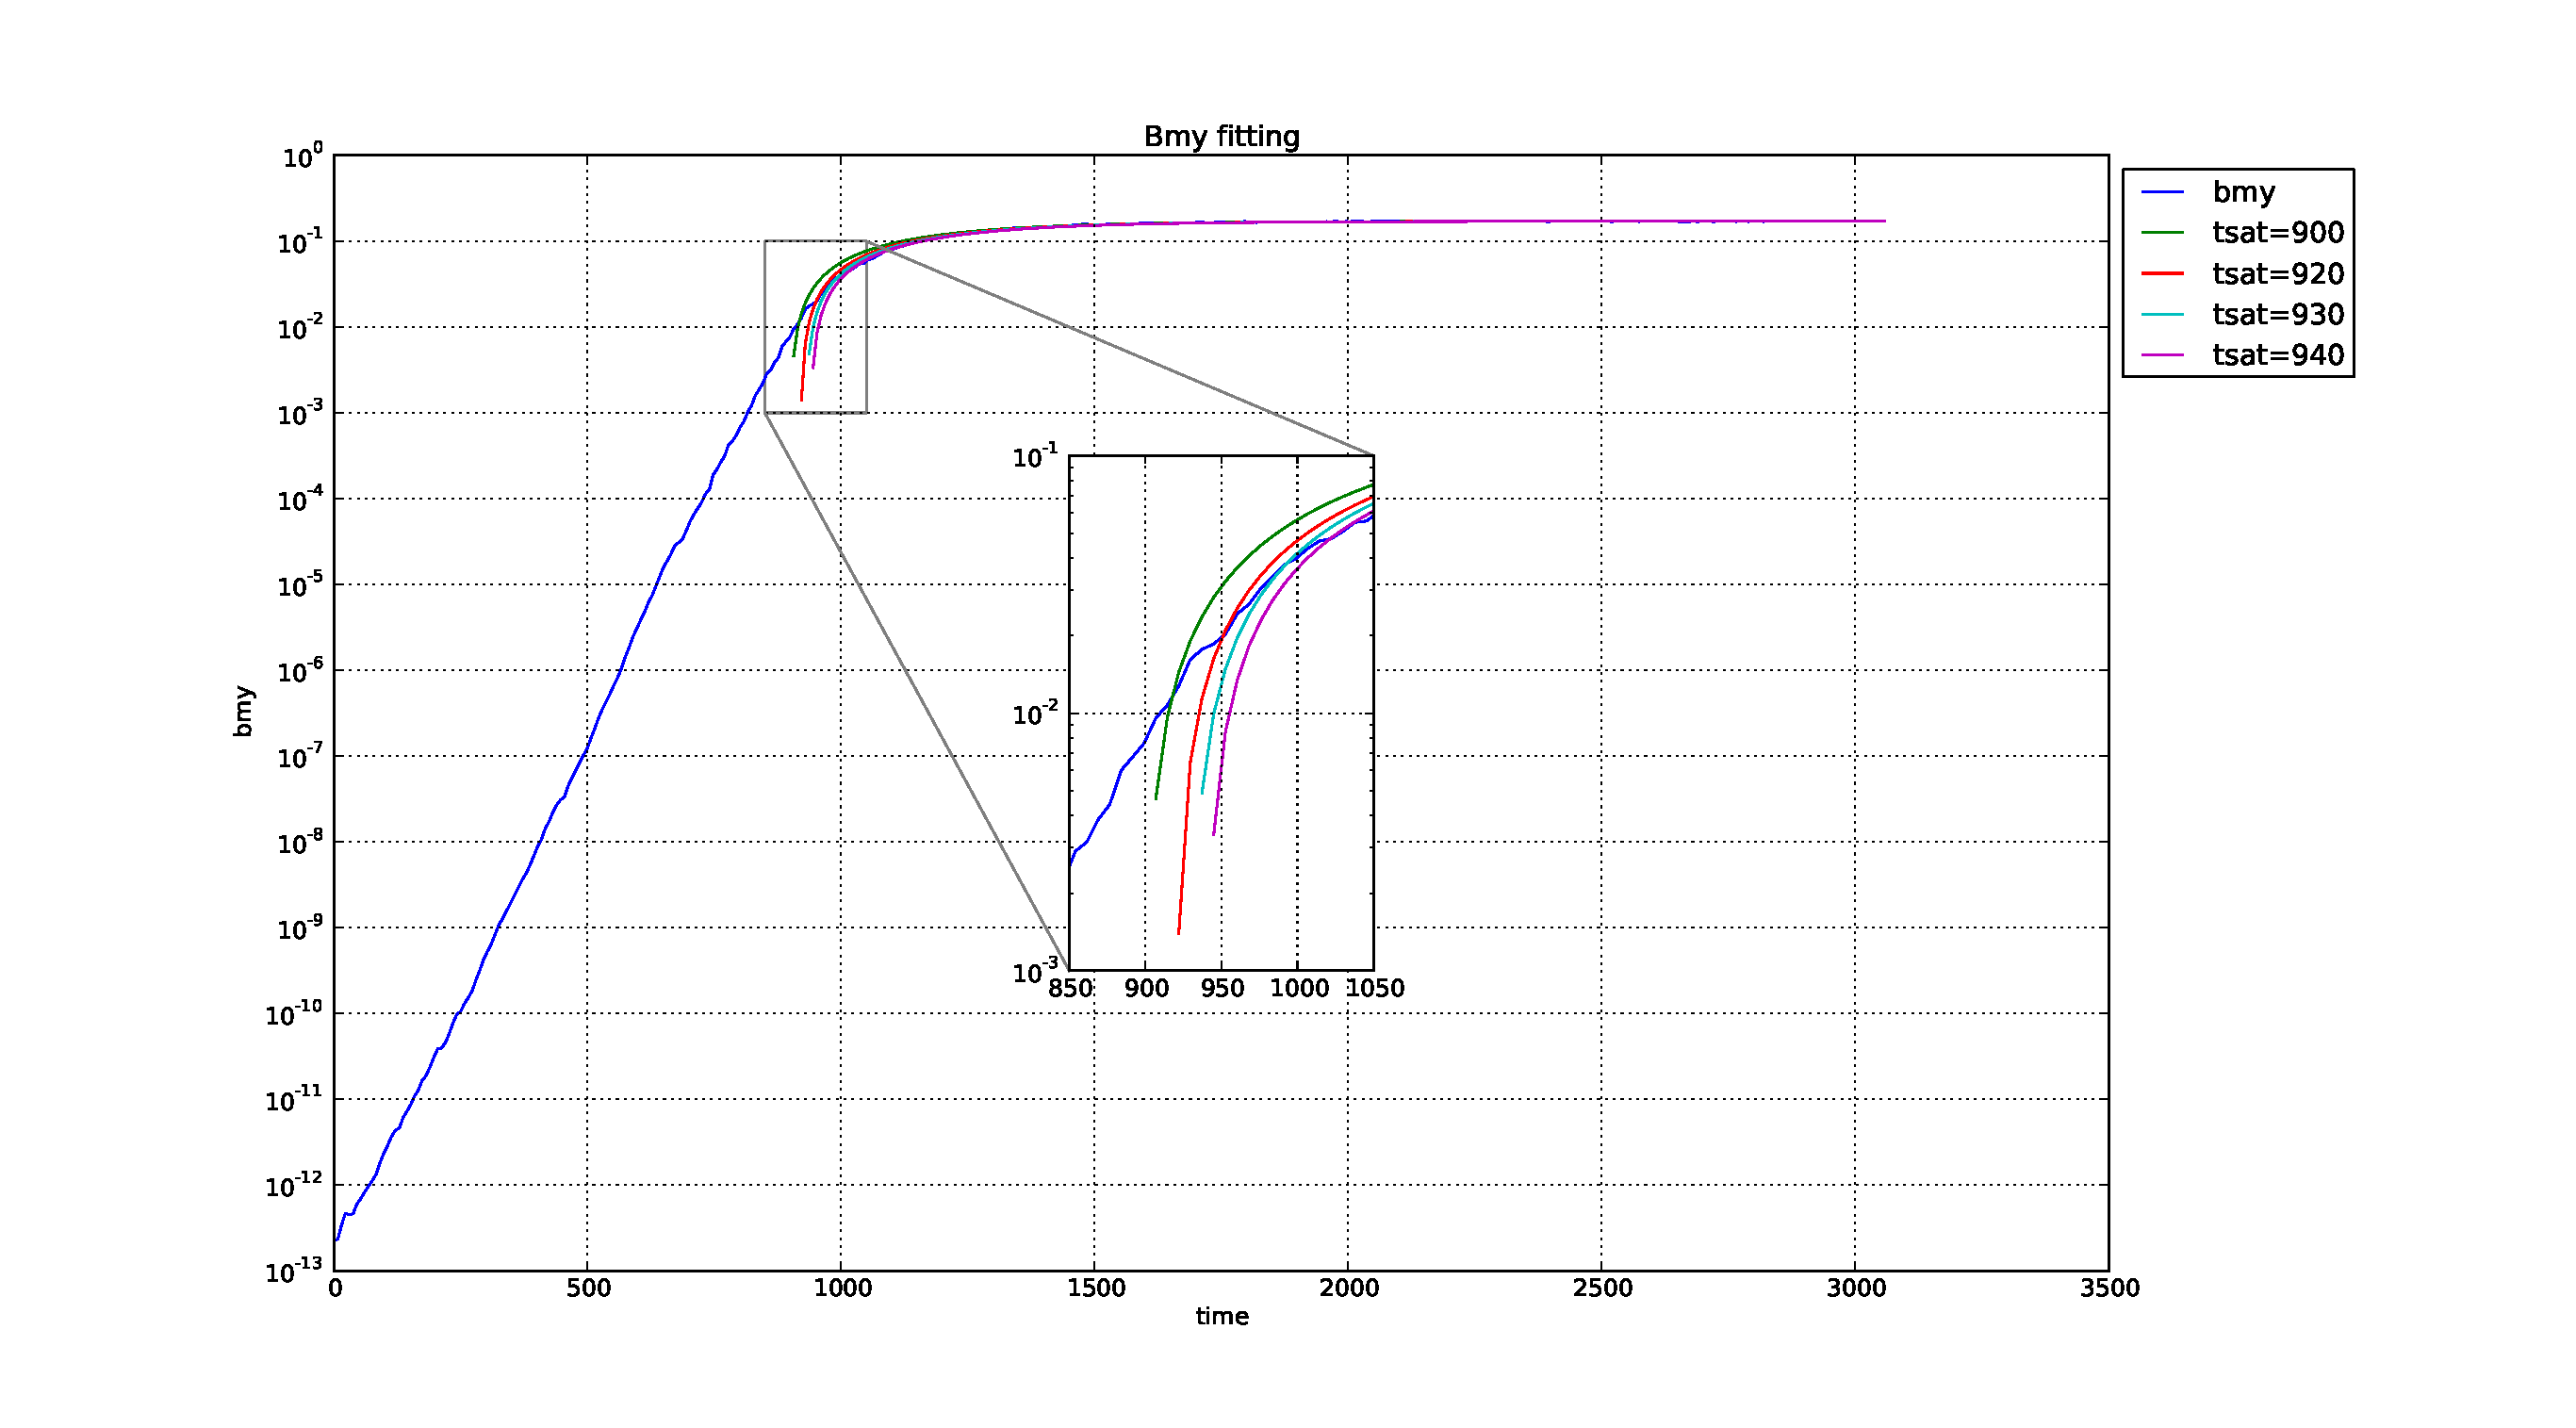
\includegraphics[width=0.8\textwidth]{bmy_fit.eps}
\caption{Bmy Fitting: $B_0=0.1712$ and $t_s = 930$.}
\label{fig:bmy_fit}
 \end{figure}
A rough fit for the field average takes the values $B_0=0.1712$ and $t_s = 930$.
$B_0$ is the saturation field value and $t_s$ is the best fit curve just before saturation.

In order to do a best mathematical fit a likelihood method could be used: 
\begin{itemize}
 \item Compute the function:
\begin{equation}
 G(t_s) = \sum_{t=a}^b (<\bar{B}^2_{(t)}>-F(t;B_0,t_s))
\end{equation}
\item Find the $t_s$ value which minimizes this function, using, for example, the false position method.

\end{itemize}
